\chapter{Технологическая часть}

\section{Выбор средств реализации}

Для реализации системы выбран гибридный подход с использованием языков C++ и Python. C++ применяется для вычислительного модуля трассировки лучей, так как обеспечивает высокую производительность при работе с большими объемами данных ($10^7$ лучей и более) и позволяет эффективно использовать вычислительные ресурсы процессора. Python используется для интерфейсной части и управления данными, так как предоставляет богатые возможности для быстрой разработки графического интерфейса и упрощает работу с библиотеками визуализации. Использование pybind11 позволило достичь производительности C++ при расчете $10^7$ лучей, сохранив гибкость Python при разработке GUI на Tkinter. C++ модуль реализован на стандарте C++17 \cite{11}, Python интерфейс использует Python 3.12 \cite{12}.

\textbf{pybind11} применен для создания модуля \texttt{cpp\_renderer}, экспортирующего классы \texttt{Renderer}, \texttt{Shield} и связанные структуры данных в Python \cite{13}. Библиотека pybind11 позволяет проводить вычисления с высокой скоростью, обеспечивая прямой доступ к C++ коду из Python без накладных расходов на сериализацию данных.

\textbf{Tkinter} применен для реализации пользовательского интерфейса. Выбор обоснован необходимостью создания легкого кроссплатформенного инструмента: библиотека входит в стандартную поставку Python, что исключает дополнительные зависимости и упрощает развертывание на различных платформах; функциональности достаточно для требуемого интерфейса без избыточных возможностей более современных фреймворков (PyQt/PySide), что снижает сложность разработки и сборки.

\textbf{Pillow (PIL)} применен для конвертации массивов данных карт освещенности в изображения для отображения в интерфейсе (через \texttt{ImageTk}) и сохранения результатов расчета \cite{15}.

\textbf{NumPy} используется как промежуточный буфер для передачи данных между C++ и PIL без копирования памяти \cite{14}.

\textbf{Matplotlib} применен в исследовательском модуле для визуализации распределения освещенности и анализа результатов расчета (интеграция с Tkinter через \texttt{FigureCanvasTkAgg}).

\section{Структура программного комплекса}

Структура проекта организована следующим образом:

\begin{itemize}
    \item \texttt{backend/} --- C++ модуль трассировки лучей;
    \begin{itemize}
        \item \texttt{src/} --- исходные файлы C++;
        \item \texttt{include/} --- заголовочные файлы;
        \item \texttt{CMakeLists.txt} --- конфигурация сборки.
    \end{itemize}
    \item \texttt{python\_app/} --- Python приложение.
    \begin{itemize}
        \item \texttt{*.py} --- модули приложения;
        \item \texttt{report/} --- результаты исследований.
    \end{itemize}
\end{itemize}

\subsection{Общая архитектура системы}

Система разделена на два основных компонента: интерфейсную часть (Python) и вычислительный модуль (C++). Такое разделение обеспечивает четкое разграничение ответственности: интерфейсная часть отвечает за взаимодействие с пользователем и управление данными, а вычислительный модуль --- за выполнение ресурсоемких операций трассировки лучей.

Модульная организация компонентов:
\begin{itemize}
    \item каждый модуль имеет четко определенную область ответственности;
    \item модули взаимодействуют через четко определенные интерфейсы;
    \item изменения в одном модуле не требуют модификации других модулей (при соблюдении интерфейсов);
    \item вычислительный модуль может быть использован независимо от интерфейсной части (например, для пакетной обработки).
\end{itemize}

Потоки данных между компонентами:
\begin{enumerate}
    \item пользователь изменяет параметры сцены через графический интерфейс;
    \item Python-код преобразует данные в структуры, понятные C++ модулю;
    \item C++ модуль выполняет расчет освещения и возвращает массивы данных;
    \item Python-код преобразует результаты в изображения и отображает их пользователю.
\end{enumerate}

\subsection{Диаграмма компонентов (UML)}

На рисунке \ref{fig:components} представлена диаграмма компонентов системы, показывающая архитектуру решения и взаимодействие между основными модулями системы.

\begin{figure}[H]
\centering
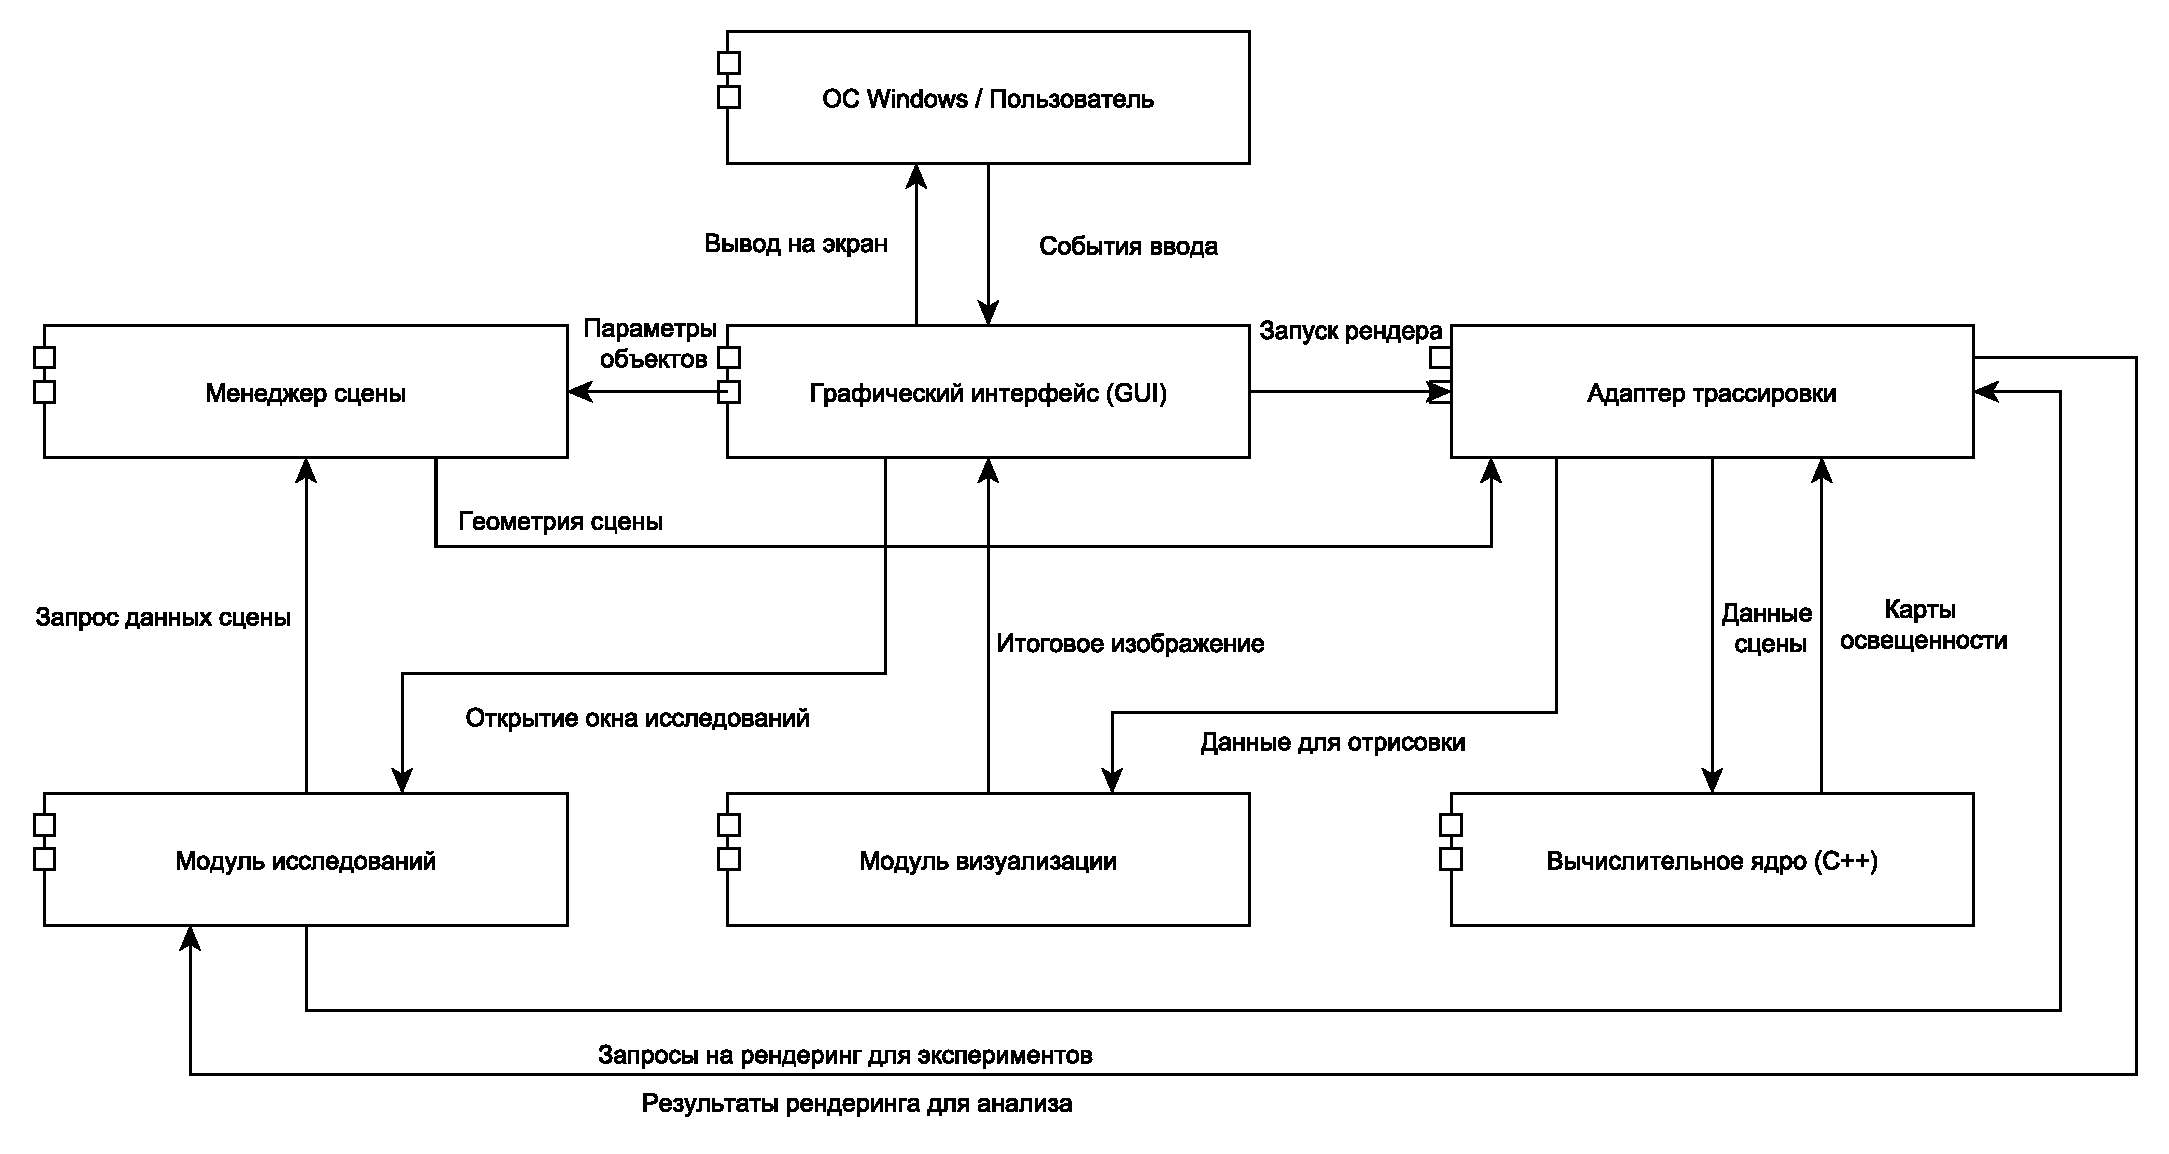
\includegraphics[width=1\textwidth]{images/components.pdf}
\caption{Диаграмма компонентов системы}
\label{fig:components}
\end{figure}

Диаграмма компонентов отражает архитектурное решение системы, разделяющее функциональность на логические модули с четко определенными интерфейсами взаимодействия.

\subsection{Описание назначения основных классов и функций}

\textbf{Модуль пользовательского интерфейса} (\texttt{gui.py}): создание и управление главным окном приложения, отображение панелей управления, визуализация результатов расчета, управление орбитальной камерой, координация работы между редактором сцены и модулем визуализации.

\textbf{Модуль редактирования сцены} (\texttt{editor.py}): инструменты для создания и редактирования конфигурации гирлянды, создание паттернов (точка, линия, дуга, круг), редактирование параметров источников света и колпачков, управление объектами сцены.

\textbf{Модуль управления сценой} (\texttt{scene.py}): управление состоянием сцены, хранение списка источников света и объектов, единый интерфейс доступа к данным, координация обновлений при изменении конфигурации.

\textbf{Модуль трассировки лучей} (\texttt{ray\_tracer.py}): высокоуровневый интерфейс для работы с C++ модулем, преобразование Python объектов в структуры C++, вызов функций расчета освещения, преобразование результатов для визуализации, управление параметрами расчета.

\textbf{Модуль визуализации} (встроен в \texttt{gui.py}): отображение результатов расчета, преобразование карт освещенности в изображения, визуализация вида камеры с использованием предрассчитанных карт.

\textbf{Модуль исследовательских инструментов} (\texttt{research.py}): дополнительные инструменты для анализа, исследование преломления (анализ влияния коэффициента преломления на форму светового пятна), исследование рассеивания (анализ влияния матовости), тестирование производительности (зависимость времени расчета от количества источников, объектов, разрешения карт).

\subsection{Модели данных}

Структуры данных определены в C++ модуле и экспортируются в Python через pybind11. Передача данных между Python и C++ выполняется через структуры (struct), автоматически преобразуемые pybind11 без копирования примитивных типов. Вложенные структуры (например, \texttt{ShieldConfig} внутри \texttt{LightConfig}) передаются как единый объект.

\textbf{Представление источников света:} структура \texttt{LightConfig} (C++) / \texttt{LightSource} (Python) содержит позицию $(x, y, z)$ как массив float[3], цвет RGB как массив float[3] в диапазоне $[0, 1]$, интенсивность (float), наличие колпачка (bool), параметры колпачка (\texttt{ShieldConfig}), количество лучей (int). Передача через pybind11 структуру обеспечивает автоматическое преобразование типов без сериализации.

\textbf{Представление объектов сцены:} стена (\texttt{WallConfig}) содержит размеры (float[2]), расстояние от начала координат (float), разрешение карты освещенности (int). Сферы (\texttt{SphereConfig}) содержат центр (float[3]), радиус (float), разрешение карты освещенности (int). Массивы координат передаются как std::array<float, N> в C++, автоматически преобразуемые pybind11 в Python tuple или numpy array.

\textbf{Представление защитных колпачков:} структура \texttt{ShieldConfig} содержит радиус внешней сферы (float), цвет RGB для фильтрации (float[3]), показатель преломления (float), прозрачность $[0, 1]$ (float), параметр рассеивания (float), радиус внутренней сферы (float). Все параметры передаются как плоские поля структуры, что обеспечивает эффективный доступ в C++ без разыменования указателей.

\textbf{Представление камеры:} структура \texttt{CameraConfig} содержит позицию (float[3]), направление взгляда (float[3]), вектор вверх (float[3]), поле зрения (float), разрешение изображения (int[2]), количество сэмплов на пиксель (int). Векторы передаются как std::array<float, 3>, что обеспечивает выравнивание данных и эффективный доступ в C++.

\textbf{Представление карт освещенности:} карты освещенности передаются как numpy массивы (numpy.ndarray) типа float32 с формой (height, width, 3) для RGB компонент. pybind11 обеспечивает прямой доступ к памяти массива без копирования через buffer protocol. Значения хранятся в диапазоне $[0, +\infty)$, при визуализации нормализуются с учетом экспозиции.

\section{Особенности реализации}

Основные алгоритмы системы реализованы в C++ модуле. Листинги кода представлены в приложении, ниже приведены описания ключевых фрагментов.

\subsubsection{Функция расчета преломления луча}

Функция \texttt{refract\_dir} (см. листинг \ref{lst:refract_dir}, файл \texttt{backend/src/renderer.cpp}, строки 18--30) обрабатывает полное внутреннее отражение через проверку дискриминанта $\eta^2 (1 - \cos^2(\theta_1))$ до вычислений, обеспечивая численную стабильность. Косинус угла падения вычисляется один раз через скалярное произведение $\cos(\theta_1) = -\vec{d} \cdot \vec{n}$, исключая тригонометрические функции.

\subsubsection{Функция аппроксимации Френеля}

Функция \texttt{fresnel\_schlick} (см. листинг \ref{lst:fresnel_schlick}, файл \texttt{backend/src/renderer.cpp}, строки 32--42) использует аппроксимацию Шлика (погрешность менее 1\%). Коэффициент $R_0$ вычисляется один раз при нормальном падении. Степень $(1 - \cos(\theta))^5$ реализована через последовательное возведение в квадрат и умножение.

\subsubsection{Обработка преломления в колпачке}

Метод \texttt{Shield::process} (см. листинг \ref{lst:shield_process}, файл \texttt{backend/src/renderer.cpp}, строки 160--228) обрабатывает пересечения с двумя концентрическими сферами через сортировку точек по параметру $t$ для определения порядка входа и выхода. Ранний выход при полном внутреннем отражении на первой границе исключает вычисления для второй сферы. Стохастическое рассеивание реализовано добавлением нормально распределенного шума с последующей нормализацией.

\subsubsection{Ядро трассировки лучей}

Метод \texttt{Renderer::trace\_ray} (см. листинг \ref{lst:trace_ray}, файл \texttt{backend/src/renderer.cpp}, строки 462--536) использует единый интерфейс проверки пересечений для всех типов объектов. Выбирается пересечение с минимальным параметром $t$ для обработки случаев множественных пересечений. Атомарное накопление интенсивности минимизирует промахи кэша. Проверка знака $\vec{n} \cdot (-\vec{d})$ исключает запись освещения на обратную сторону поверхности.

\section{Тестирование корректности}

\subsection{Методы верификации ПО}

Для проверки работоспособности использовались методы тестирования: черный ящик (проверка основных функций) и белый ящик (проверка корректности алгоритмов).

\subsection{Примеры работы программы на разных данных}

\subsubsection{Корректные данные}

Программа успешно обрабатывает различные конфигурации сцен:

\begin{itemize}
    \item различные конфигурации источников света: программа корректно обрабатывает сцены с количеством источников от 1 до 100 и более. Все источники света правильно учитываются при расчете освещения;
    
    \item различные параметры колпачков: система корректно обрабатывает колпачки с различными коэффициентами преломления (от 1.0 до 2.0), прозрачностью (от 0.0 до 1.0) и параметрами рассеивания. Преломление света рассчитывается физически корректно;
    
    \item различные геометрии сцен: программа успешно обрабатывает сцены с различным количеством объектов (сфер) от 0 до 20 и более. Карты освещенности формируются корректно для всех поверхностей.
\end{itemize}

\subsubsection{Некорректные данные}

Программа корректно обрабатывает ошибки при некорректных входных данных:

\begin{itemize}
    \item граничные значения: при указании нулевого или отрицательного количества лучей, нулевого разрешения карт освещенности система выдает информативные сообщения об ошибках;
    
    \item некорректные параметры: при указании некорректных значений параметров (например, отрицательный радиус сферы, некорректные координаты) система проверяет входные данные и выдает предупреждения;
    
    \item поведение при граничных значениях: система стабильно работает при максимальных значениях параметров (большое количество источников, объектов, высокое разрешение).
\end{itemize}

\section{Руководство пользователя}

\subsection{Интерфейс программы}

На рисунке \ref{fig:gui_main} представлен главный интерфейс программы. Главное окно объединяет все основные элементы интерфейса:
\begin{itemize}
    \item редактор гирлянды (слева): интерактивный холст для размещения источников света и объектов сцены, инструменты создания паттернов (точка, линия, дуга, круг, сфера), схемы сцены (вид сверху и покрытие стены);
    \item область визуализации (справа): отображение результатов расчета освещения на стене, настройки рендеринга (количество лучей, сэмплы камеры, режим распределения лучей), управление камерой (орбитальный просмотр), настройки экспозиции;
    \item кнопки управления: рендеринг сцены, сохранение изображения, открытие окна исследований.
\end{itemize}

\begin{figure}[H]
\centering
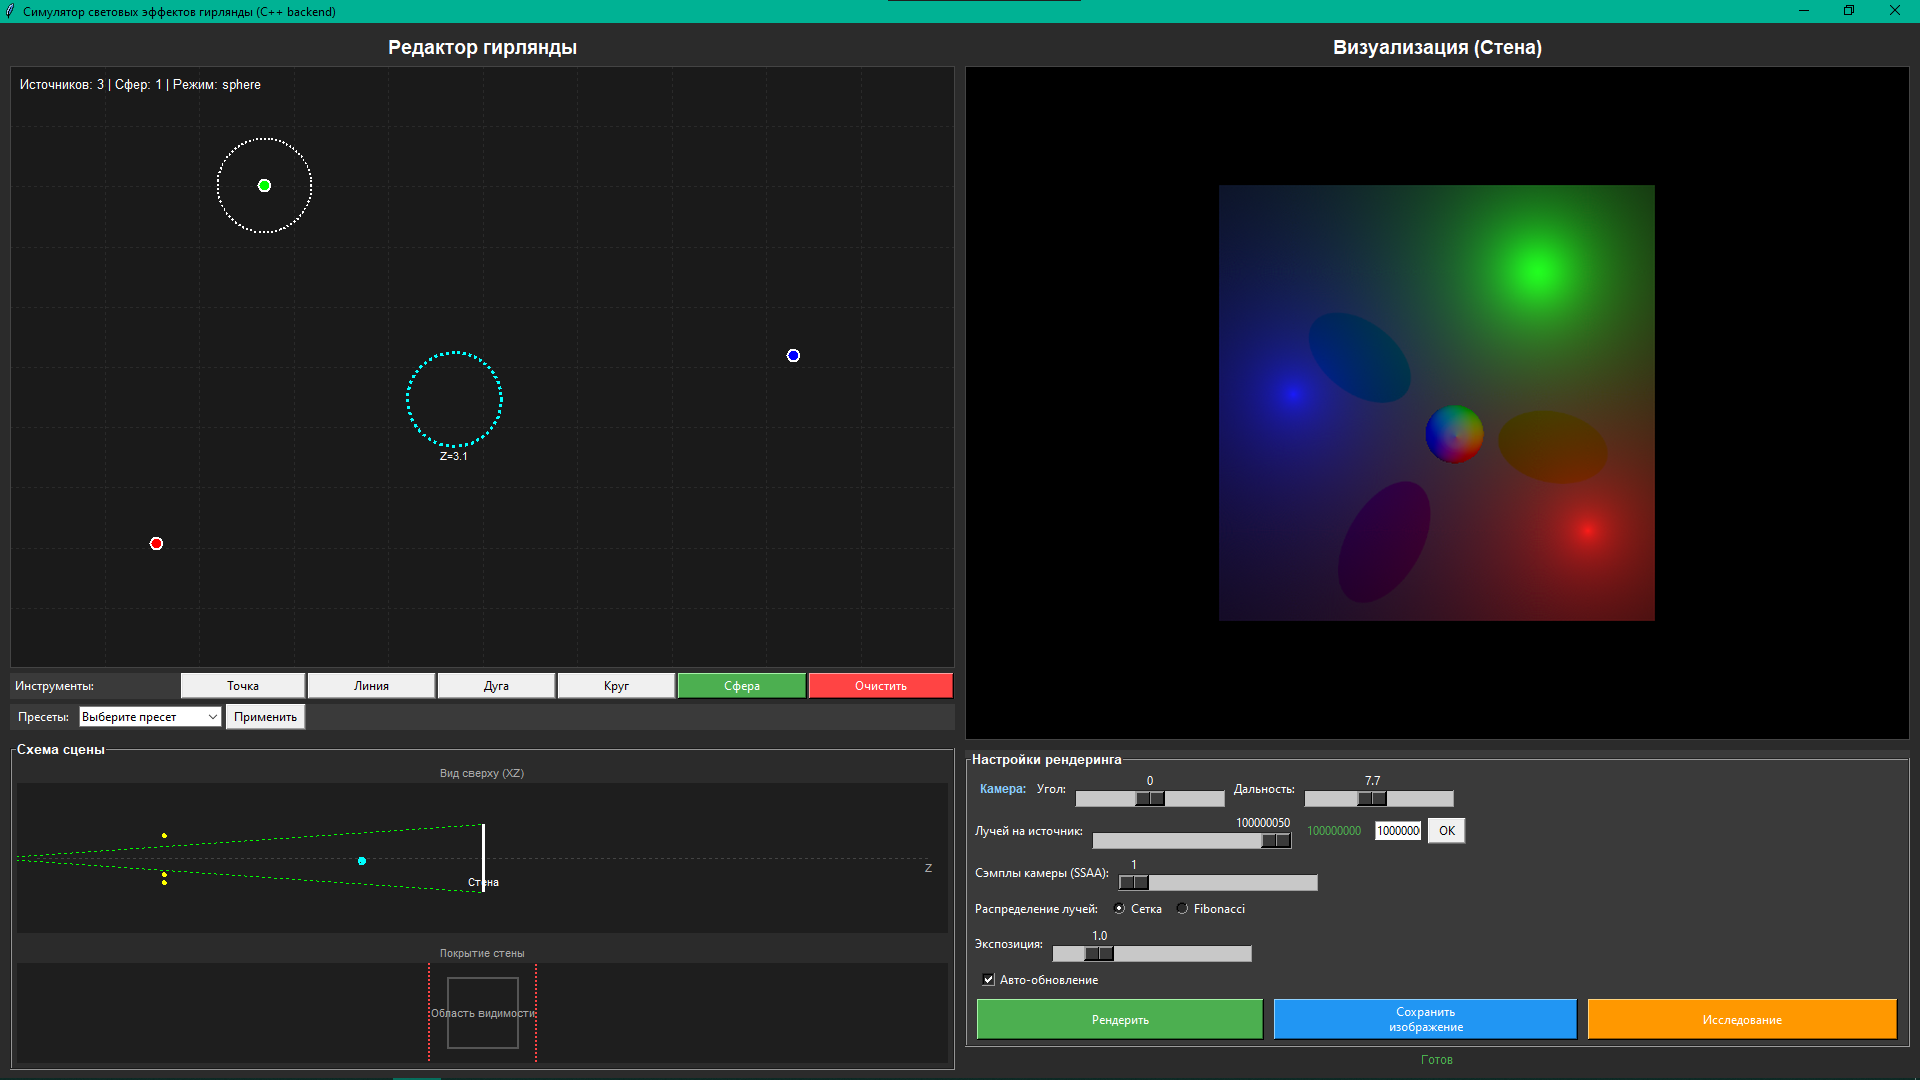
\includegraphics[width=0.9\textwidth]{images/gui_main.png}
\caption{Главное окно приложения}
\label{fig:gui_main}
\end{figure}

На рисунке \ref{fig:gui_shield_settings} представлено модальное окно настройки параметров защитного колпачка источника света.

\begin{figure}[H]
\centering
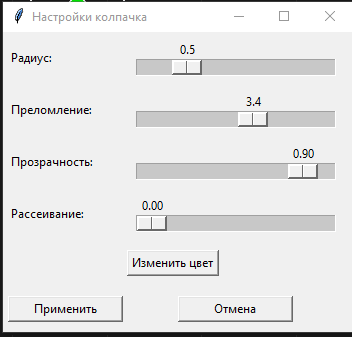
\includegraphics[width=0.6\textwidth]{images/gui_shield_settings.png}
\caption{Модальное окно настройки параметров колпачка}
\label{fig:gui_shield_settings}
\end{figure}

На рисунке \ref{fig:gui_research} представлено окно исследовательских инструментов. Окно предоставляет три основных инструмента анализа:
\begin{itemize}
    \item исследование преломления: анализ влияния коэффициента преломления колпачка на форму светового пятна. Генерирует серию изображений с различными значениями коэффициента преломления и профили интенсивности;
    \item исследование рассеивания: анализ влияния параметра рассеивания (матовости) на размытие светового пятна;
    \item тестирование производительности: инструмент для измерения производительности системы с настраиваемыми параметрами (тип исследования, диапазон значений, количество прогонов). Автоматически строит графики зависимости времени расчета от различных параметров.
\end{itemize}
Результаты исследований отображаются в области с прокруткой, графики автоматически сохраняются в папку \texttt{research\_results}.

\begin{figure}[H]
\centering
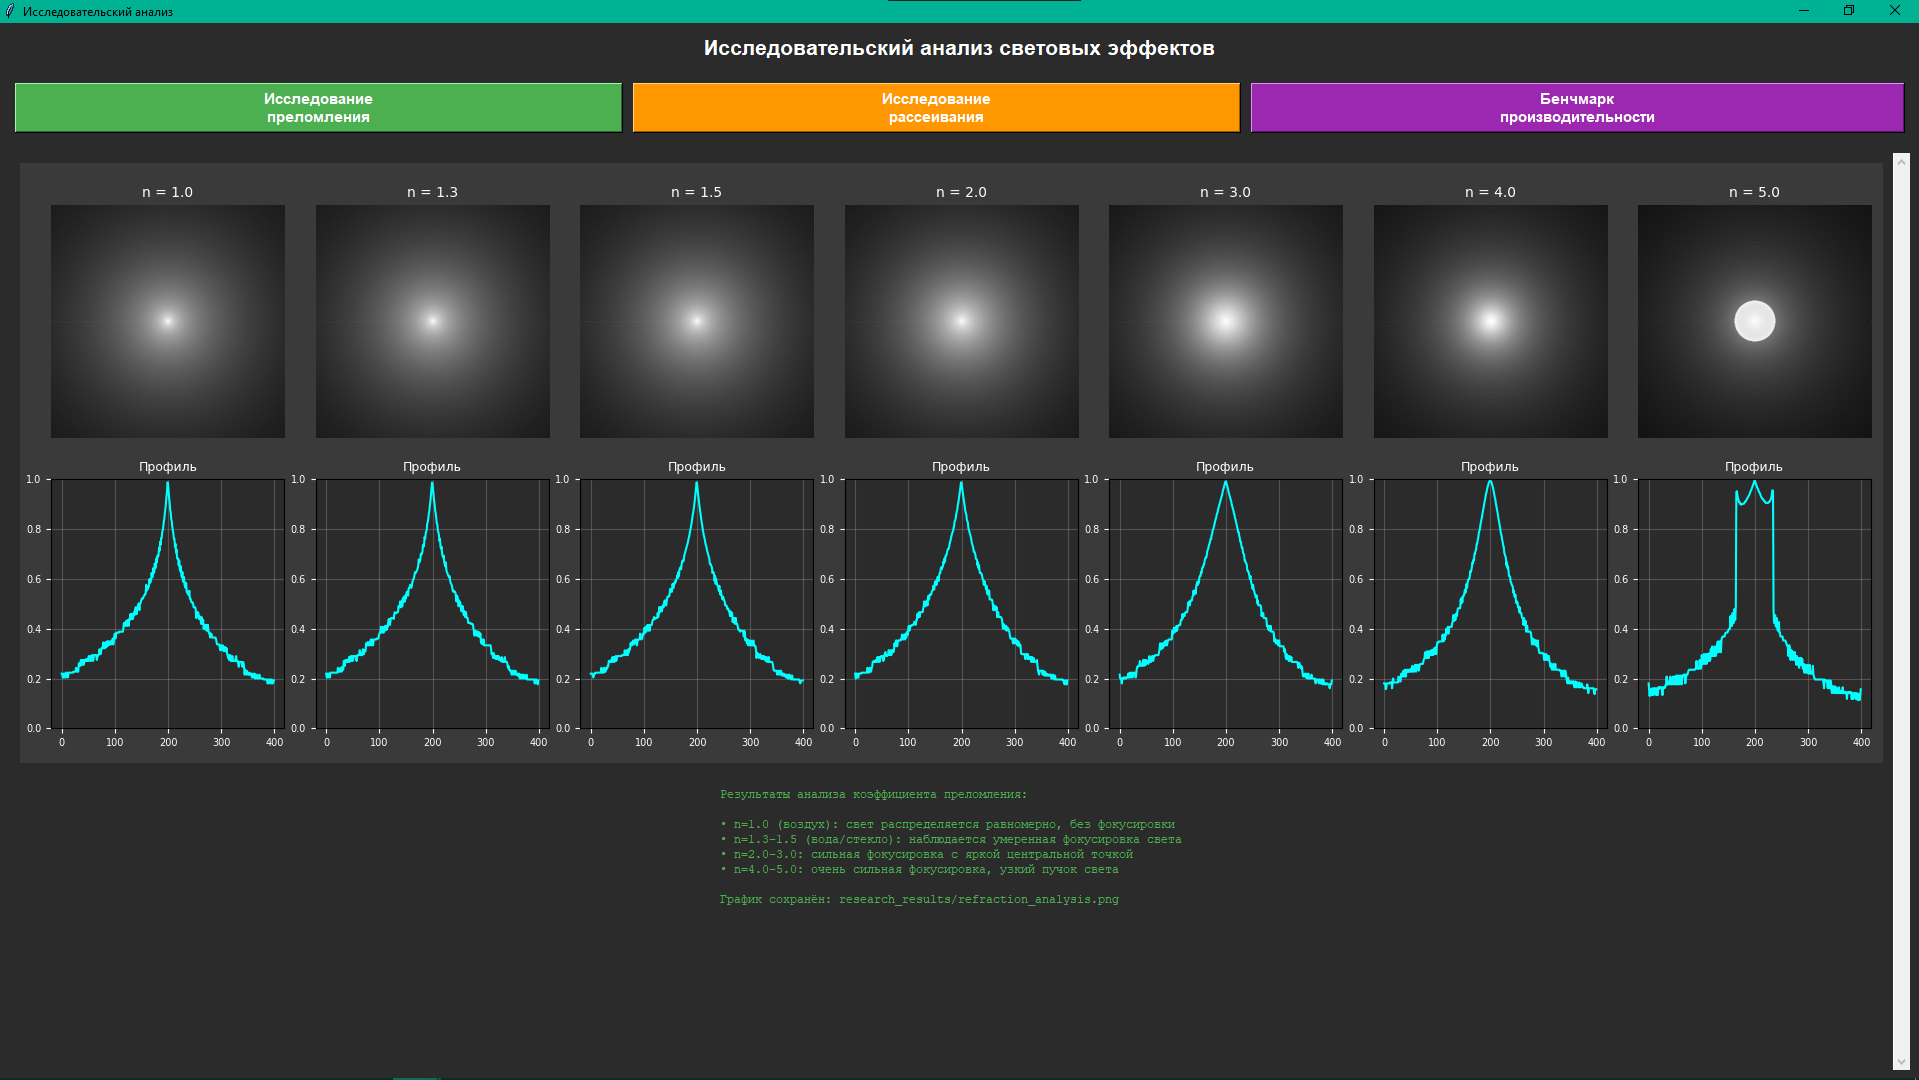
\includegraphics[width=0.9\textwidth]{images/gui_research.png}
\caption{Окно исследовательских инструментов}
\label{fig:gui_research}
\end{figure}

\subsection{Основные возможности программы}

Программа предоставляет следующие возможности:
\begin{itemize}
    \item создание паттернов источников света (точка, линия, дуга, круг, сфера);
    \item редактирование параметров источников света (позиция, цвет, интенсивность);
    \item настройка параметров защитных колпачков (коэффициент преломления, прозрачность, рассеивание, цвет);
    \item добавление объектов сцены (сферы);
    \item предварительный расчет освещения (запекание карт освещенности);
    \item интерактивный просмотр сцены с управлением камерой (орбитальный просмотр);
    \item визуализация результатов расчета с настройками экспозиции и качества;
    \item исследовательские инструменты: анализ преломления, рассеивания и тестирование производительности.
\end{itemize}


\clearpage
